\chapter{Guida utente}

La schermata iniziale dell'applicazione consiste in un'interfaccia che consente all'utente di impostare i seguenti parametri per l'avvio di una sessione di simulazione:
\begin{itemize}
\item il numero di blob, distribuiti in equa misura tra Base Blob e Cannibal Blob
\item il numero di piante, distribuite tra Standard Plant, Reproducing Plant e Poisonous Plant
\item il numero di ostacoli, distribuiti tra Base Obstacle con \code{damageEffect} e \code{slowEffect}
\item il valore della luminosità minima
\item il valore della temperatura minima
\item la durata in giornate della sessione di simulazione
\end{itemize}

Cliccando il pulsante Start si procederà all'avvio della simulazione.

\begin{figure}[h!]
\centering
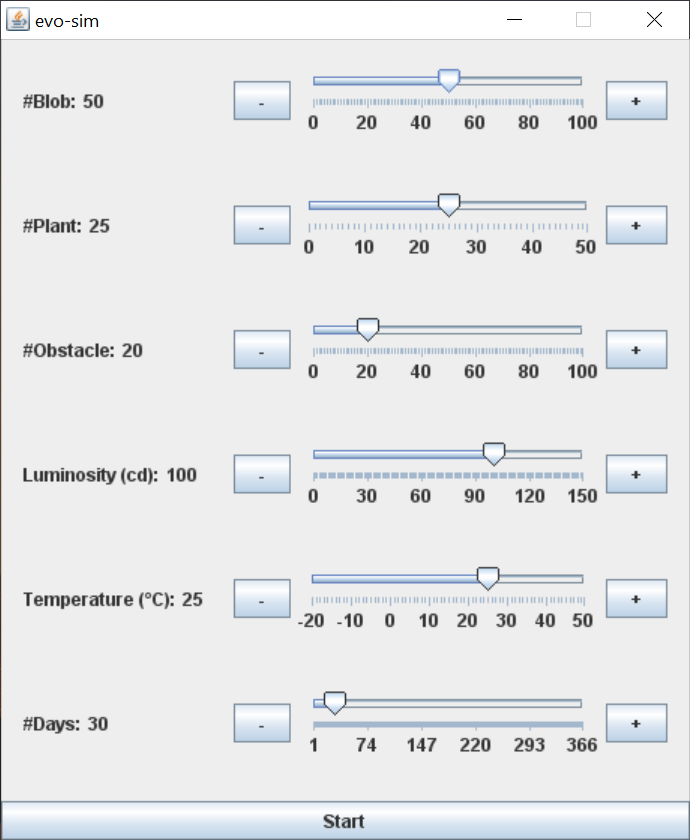
\includegraphics[scale=0.5]{img/InputInterface.png}
\caption{Schermata di input}
\label{fig:InputInterface}
\end{figure}

La schermata della simulazione è caratterizzata da una barra di indicatori in real-time e da un pannello rappresentare il mondo di della simulazione. La proprietà BoundingBox di un'entità determina la dimensione e il tipo di forma geometrica che la rappresenterà nel model:

\begin{itemize}
	\item i blob sono rappresentati da circonferenze. È rappresentata anche l'ampiezza del loro campo visivo mediante una circonferenza con perimetro di colore giallo. Il colore è determinato dal suo tipo:
	\begin{itemize}
		\item blu per i Base Blob
		\item rosso per i Cannibal Blob
		\item magenta per i Poisonous Blob
		\item grigio per gli Slow Blob
	\end{itemize}
	\item i cibi sono rappresentati da triangoli verdi. I cibi con effetto \code{standardFoodEffect} sono più piccoli dei cibi con effetto \code{poisonousFoodEffect}, e questi ultimi sono più piccoli dei cibi con effetto \code{reproducingFoodEffect};
	\item gli ostacoli sono rappresentati da rettangoli rossi. Gli ostacoli con effetto \code{damageEffect} sono più piccoli degli ostacoli con effetto \code{slowEffect};
	\item le piante sono rappresentate da rettangoli con colore dipendente dal loro tipo:
	\begin{itemize}
		\item verde per le Standard Plant
		\item rosa per le Reproducing Plant
		\item magenta per le Poisonous Plant
	\end{itemize}
\end{itemize}

Il colore di sfondo varia da blu a rosso in base al valore della temperatura corrente, e vi è un filtro nero con un valore di trasparenza dipendente dal valore di luminosità che copre le entità diverse dai blob nel caso queste non siano all'interno del loro campo visivo.

La barra degli indicatori mostra in tempo reale il giorno corrente, il numero di entità blob presenti nella simulazione e i valori di temperatura e luminosità.

\begin{figure}[h!]
\centering
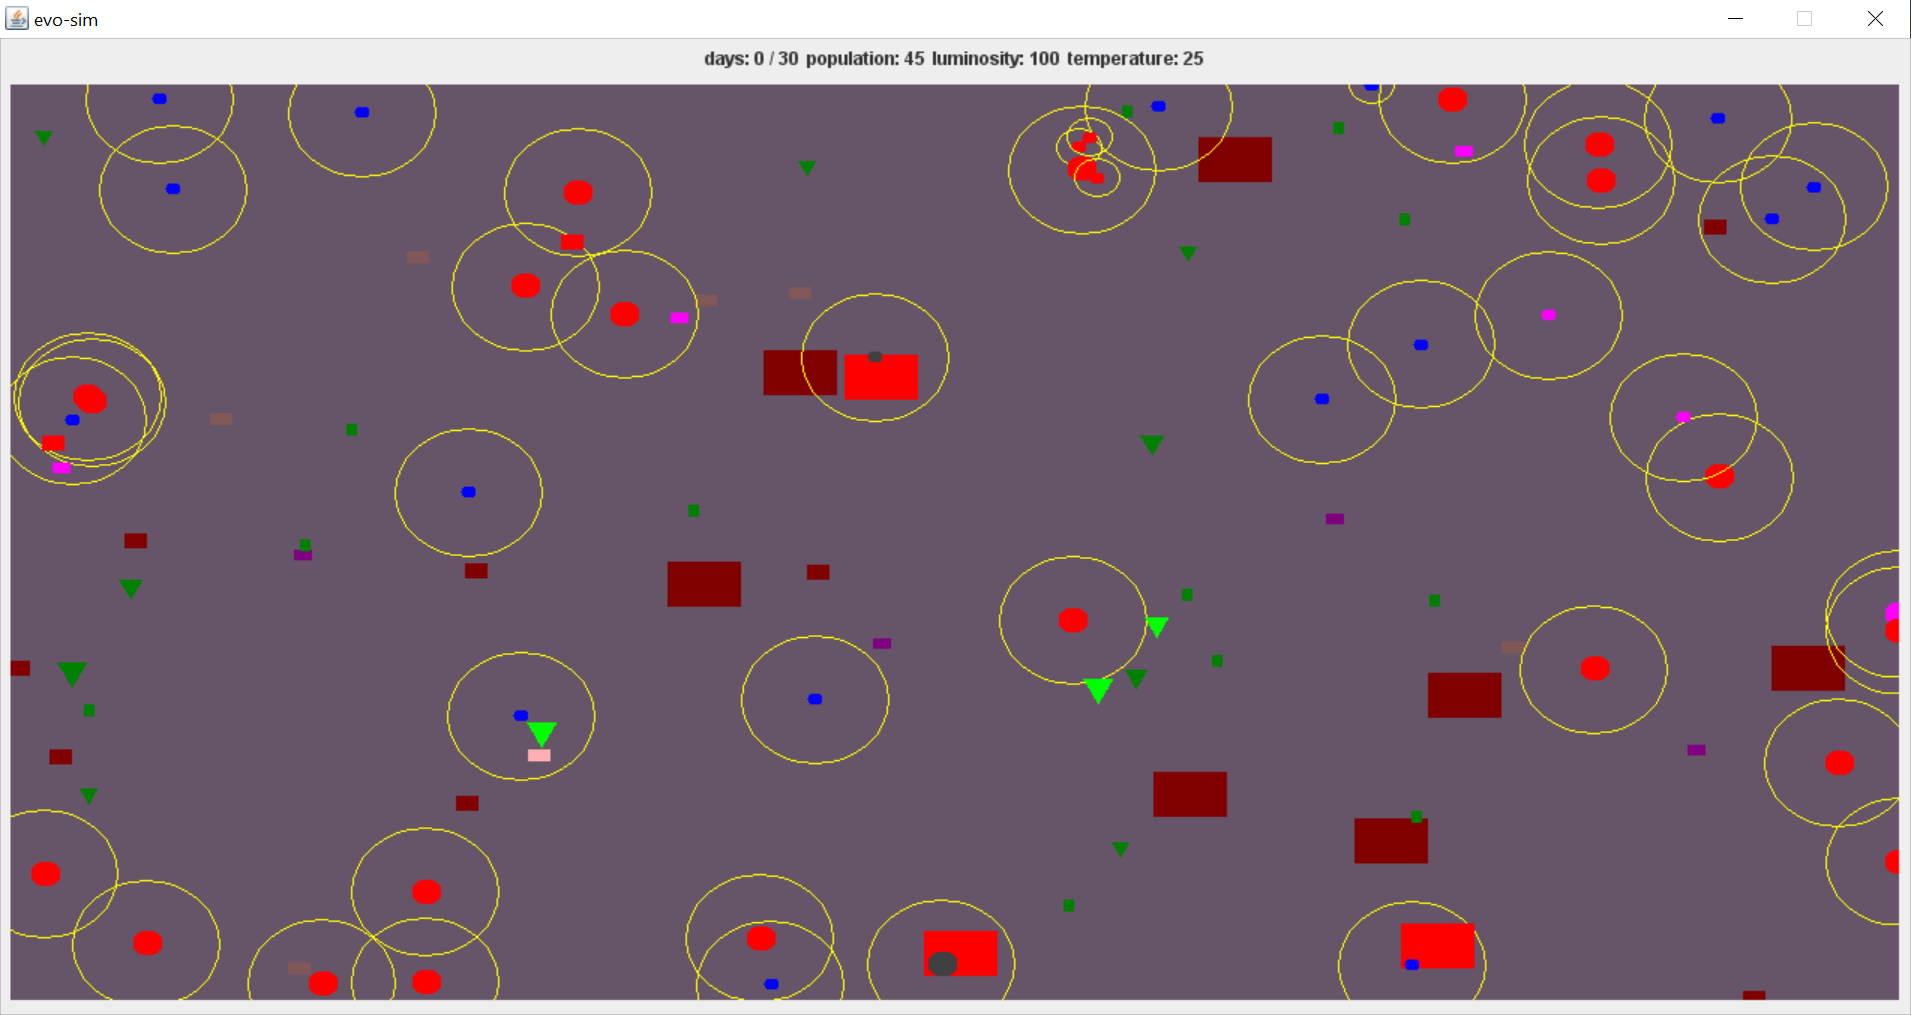
\includegraphics[width=\textwidth, scale=0.44]{img/SimulationInterface.png}
\caption{Schermata della simulazione}
\label{fig:SimulationInterface}
\end{figure}

Al termine della simulazione, verrà visualizzato un pannello con tre grafici:
\begin{itemize}
\item un istogramma raffigurante la quantità di blob e cibi presenti al termine di ciascuna giornata della simulazione
\item un grafico a torta che mostra il rapporto tra le quantità delle entità generate nel corso della simulazione per blob, cibi e ostacoli
\item un grafico a linee che mostra la media delle proprietà chiave dei blob (velocità, dimensione, campo visivo) per ciascuna giornata della simulazione
\end{itemize}

\begin{figure}[h!]
\centering
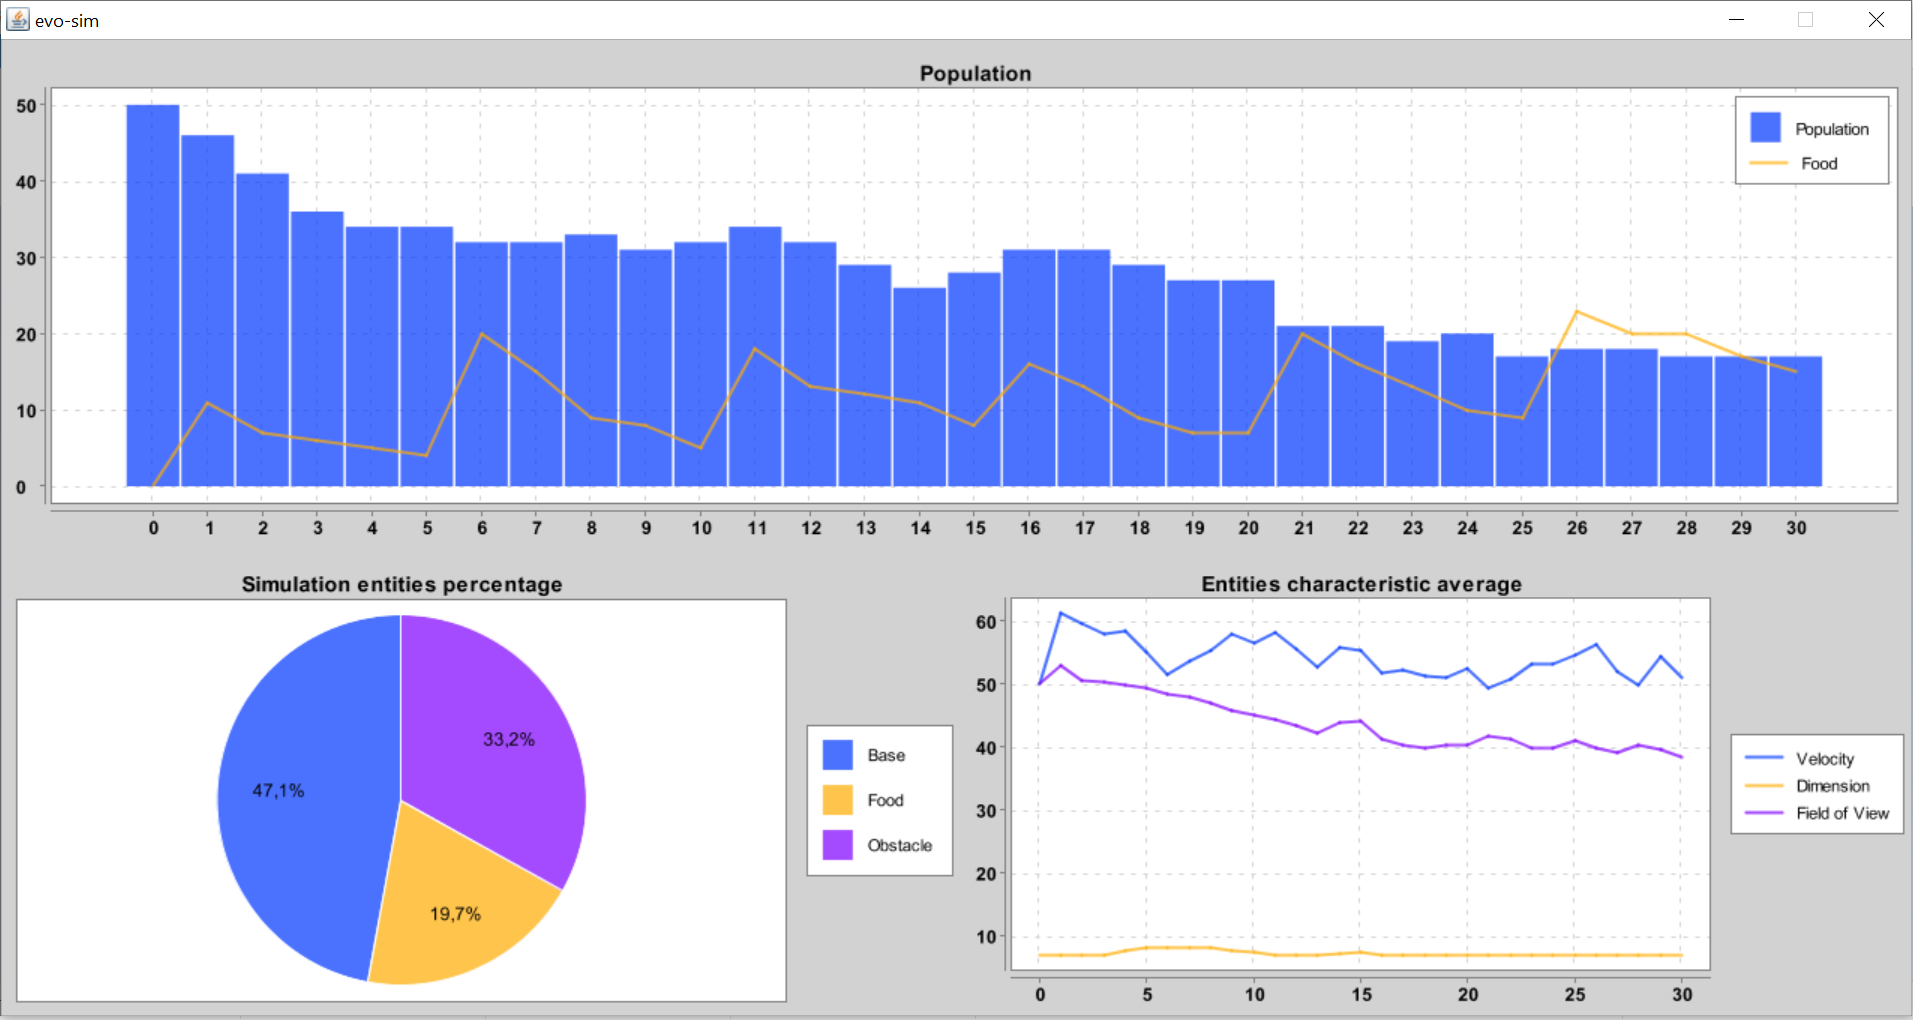
\includegraphics[width=\textwidth, scale=0.44]{img/ResultsInterface.png}
\caption{Schermata finale dei dati osservati}
\label{fig:ResultsInterface}
\end{figure}